\section{Experiments}
\label{sec:experiments}

\subsection{Questions and protocol}

We ask four questions: (Q1) Is structural utility heterogeneous enough to make
fallback necessary? (Q2) Does \method{} activate nonvacuously while avoiding
materially harmful activations? (Q3) How close is the certified policy to an
oracle that sees the evaluation sign? (Q4) How do privacy allocation and
visibility change the feasible activation region?

The confirmatory protocol, configuration hash, code commit, certificate
threshold, access gates, and random salts were frozen before the sealed
holdout was opened. Six social and blog networks were evaluated with five
seeds, producing $30$ primary dataset--seed cells. Training, certification,
and $Q5$ evaluation roles are disjoint. Hyperparameters were selected only on
the earlier validation split. The sealed test payloads were accessed once;
all commitments and accountants were independently reproduced.

\begin{table}[t]
\caption{Datasets and frozen candidate configuration. Edges are canonical
undirected edges.}
\label{tab:datasets}
\centering
\footnotesize
\setlength{\tabcolsep}{3.2pt}
\begin{tabular}{lrrrr}
\toprule
Dataset & Nodes & Edges & Features & $(r,L)$\\
\midrule
BlogCatalog & 10,312 & 333,983 & 39 & (16,2)\\
Facebook & 22,470 & 170,823 & 4,714 & (32,1)\\
PolBlogs & 1,490 & 16,715 & 2 & (8,2)\\
LastFM Asia & 7,624 & 27,806 & 7,842 & (32,1)\\
GitHub Social & 37,700 & 289,003 & 4,005 & (32,1)\\
Deezer Europe & 28,281 & 92,752 & 31,241 & (8,1)\\
\bottomrule
\end{tabular}
\end{table}

Here $r$ is projection dimension and $L$ is the number of private aggregation
hops. The public branch is sparse cosine over registered node descriptors.
The candidate averages cosine scores from the public and cached noisy
aggregation channels. It is a GAP-style adaptation, not an official GAP
reproduction. Five public home-client partitions are used. The primary
mechanism exposes individually noised client messages.

\subsection{Privacy and certificate settings}

Training and certification each target $\eps=4$ at $\delta=10^{-6}$. Their
full RDP curves are summed and converted once, yielding
$(\eps,\delta)=(5.6640,2\times10^{-6})$. The material threshold is
$\gamma=0.02$, minimum private lower count is $50$, and failure allocations
are $(\beta_S,\beta_n,\beta_{\mathrm{stat}})=(0.01,0.01,0.03)$.
The diagnostic grid contains $5$ training budgets, $5$ certification budgets,
$2$ visibility models, $6$ datasets, and $5$ seeds ($1500$ records).
Every grid cell is a counterfactual deployment, not a jointly released
mechanism.

\subsection{Primary result}

\begin{figure*}[t]
  \centering
  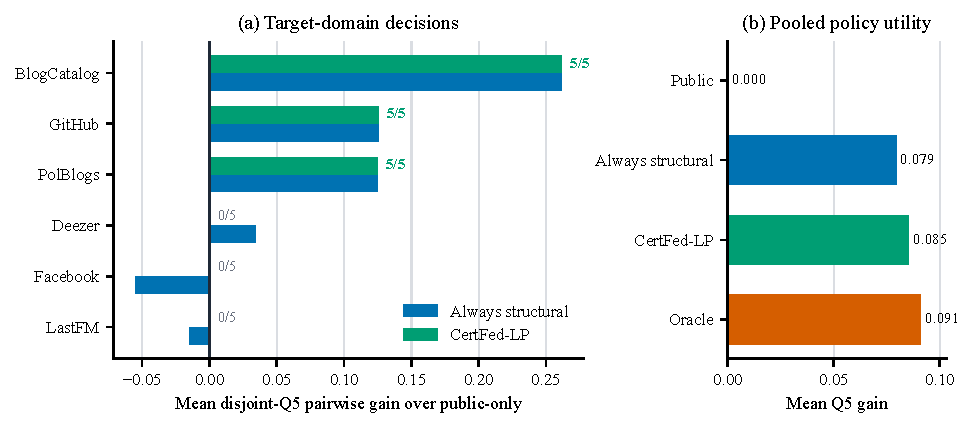
\includegraphics[width=\textwidth]{figures/figure2_primary_policy.pdf}
  \caption{Primary visible-message result at composed
  $(\eps,\delta)=(5.6640,2\times10^{-6})$. (a) Mean disjoint-$Q5$ pairwise
  advantage of always enabling the structural branch; green overlays indicate
  the gain retained by \method{}, with activation counts shown per dataset.
  (b) Pooled policy gain over public-only. The oracle uses the $Q5$ sign and is
  not deployable.}
  \label{fig:primary}
\end{figure*}

\begin{table}[t]
\caption{Preregistered primary result over five seeds. ``Full'' is the finite
holdout candidate advantage; ``Policy'' is disjoint-$Q5$ gain after the
private decision.}
\label{tab:primary}
\centering
\footnotesize
\setlength{\tabcolsep}{3.2pt}
\begin{tabular}{lrrrr}
\toprule
Dataset & Activate & Full & Policy & AUC pol.\\
\midrule
BlogCatalog & 5/5 & +0.2621 & +0.2618 & +0.3320\\
GitHub Social & 5/5 & +0.1260 & +0.1257 & +0.1948\\
PolBlogs & 5/5 & +0.1254 & +0.1251 & +0.1757\\
Deezer Europe & 0/5 & +0.0337 & 0.0000 & 0.0000\\
Facebook & 0/5 & $-$0.0543 & 0.0000 & 0.0000\\
LastFM Asia & 0/5 & $-$0.0146 & 0.0000 & 0.0000\\
\midrule
Mean / total & 15/30 & +0.0797 & \textbf{+0.0854} & +0.1171\\
\bottomrule
\end{tabular}
\end{table}

\cref{fig:primary,tab:primary} answer Q1--Q3. Structural utility changes sign:
always-structural is harmful in $10/30$ cells. \method{} activates exactly all
five seeds on BlogCatalog, GitHub Social, and PolBlogs, and falls back on
Deezer, Facebook, and LastFM. It observes zero material false activations and
has mean $Q5$ policy gain $0.08543$. The always-structural and non-deployable
oracle gains are $0.07945$ and $0.09112$, respectively, leaving mean oracle
regret $0.00568$. As a secondary standard metric, the selected policy improves
global ROC-AUC by $0.1171$ on average. Deezer is an informative abstention: its mean advantage is
positive but the mean certificate lower bound is $-0.0028<\gamma$.

\subsection{Privacy--utility phase behavior}

\begin{figure*}[t]
  \centering
  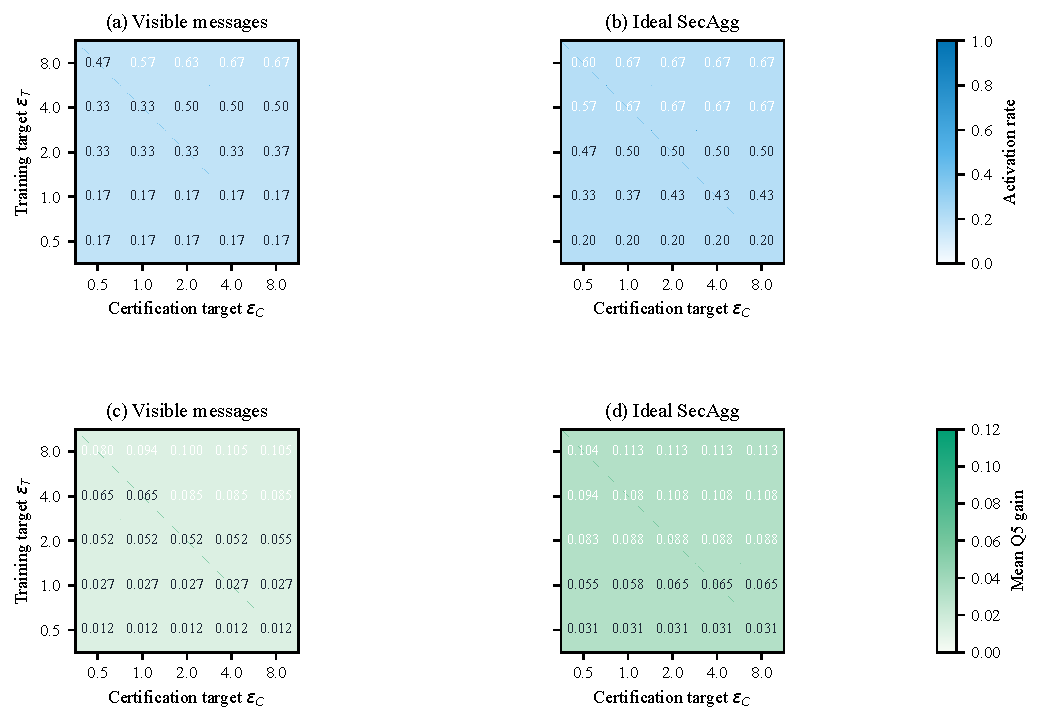
\includegraphics[width=\textwidth]{figures/figure3_privacy_phase.pdf}
  \caption{Diagnostic activation phase over training budget,
  certification budget, and visibility. Each cell reports a counterfactual
  deployment over 30 dataset--seed records. Ideal secure aggregation is a
  separate trust model and reduces aggregate noise; it is not an extra DP
  claim.}
  \label{fig:phase}
\end{figure*}

\cref{fig:phase} answers Q4. More training budget expands activation coverage.
At the primary $(4,4)$ target, visible messages activate $15$ records with
mean policy gain $0.0854$, whereas ideal aggregation activates $20$ with gain
$0.1075$. Across all $1500$ diagnostic records, no material false activation
is observed. This is descriptive evidence beyond the one frozen primary cell;
the formal error guarantee remains per deployed certificate.

\subsection{Audit and robustness checks}

The independent audit verifies $1500/1500$ unique records, all source and
split commitments, the single test-access record, no test tuning, and exact
reproduction of every stored RDP curve and converted epsilon. Original
global/intra/cross ROC-AUC values are retained only as secondary diagnostics:
the certificate and decision use the bounded pairwise estimand. Ties receive
half credit, and endpoint corruption performs no graph-dependent rejection,
preserving the stated sensitivity.
